\section{Multiplexer Silicon Results}
\label{sec:multiplexer_silicon_res}
After Tiny Tapeout 4 silicon was received and tested, the worst round trip latency was measured to be \qty{20}{\ns} as shown in Fig~\ref{fig:round_trip_latency_rising_edge} and \ref{fig:round_trip_latency_falling_edge}.

Some Tiny Tapeout 3.5 designs have been validated, including a VGA clock project (Fig.~\ref{fig:VGA_clock_design_TT03_5_silicon}) which takes advantage of the new higher speed IO.

The overhead of multiplexing multiple tiles makes power consumption of the infrastructure only a minor concern at this point. No direct comparison of the power consumption impact of the multiplexer over the previous scan chain architecture is available at the time of writing. The motivation of the multiplexer approach, however, was to substantially increase the bandwidth of the IOs.

\begin{figure}[!t]
\centering
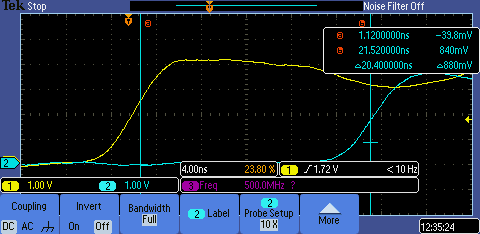
\includegraphics[width=\columnwidth]{./Figs/tt3p5 rising latency.PNG}
\caption{The Tiny Tapeout 3.5 round trip latency on a rising edge, measured at about \qty{20}{\ns}.}
\label{fig:round_trip_latency_rising_edge}
\end{figure}

\begin{figure}[!t]
\centering
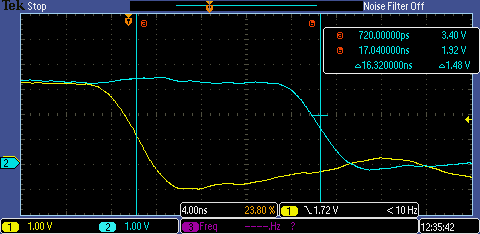
\includegraphics[width=\columnwidth]{./Figs/tt3p5 falling latency.PNG}
\caption{The Tiny Tapeout 3.5 round trip latency on a falling edge, measured at about \qty{16}{\ns}.}
\label{fig:round_trip_latency_falling_edge}
\end{figure}

\begin{figure}[!t]
\centering
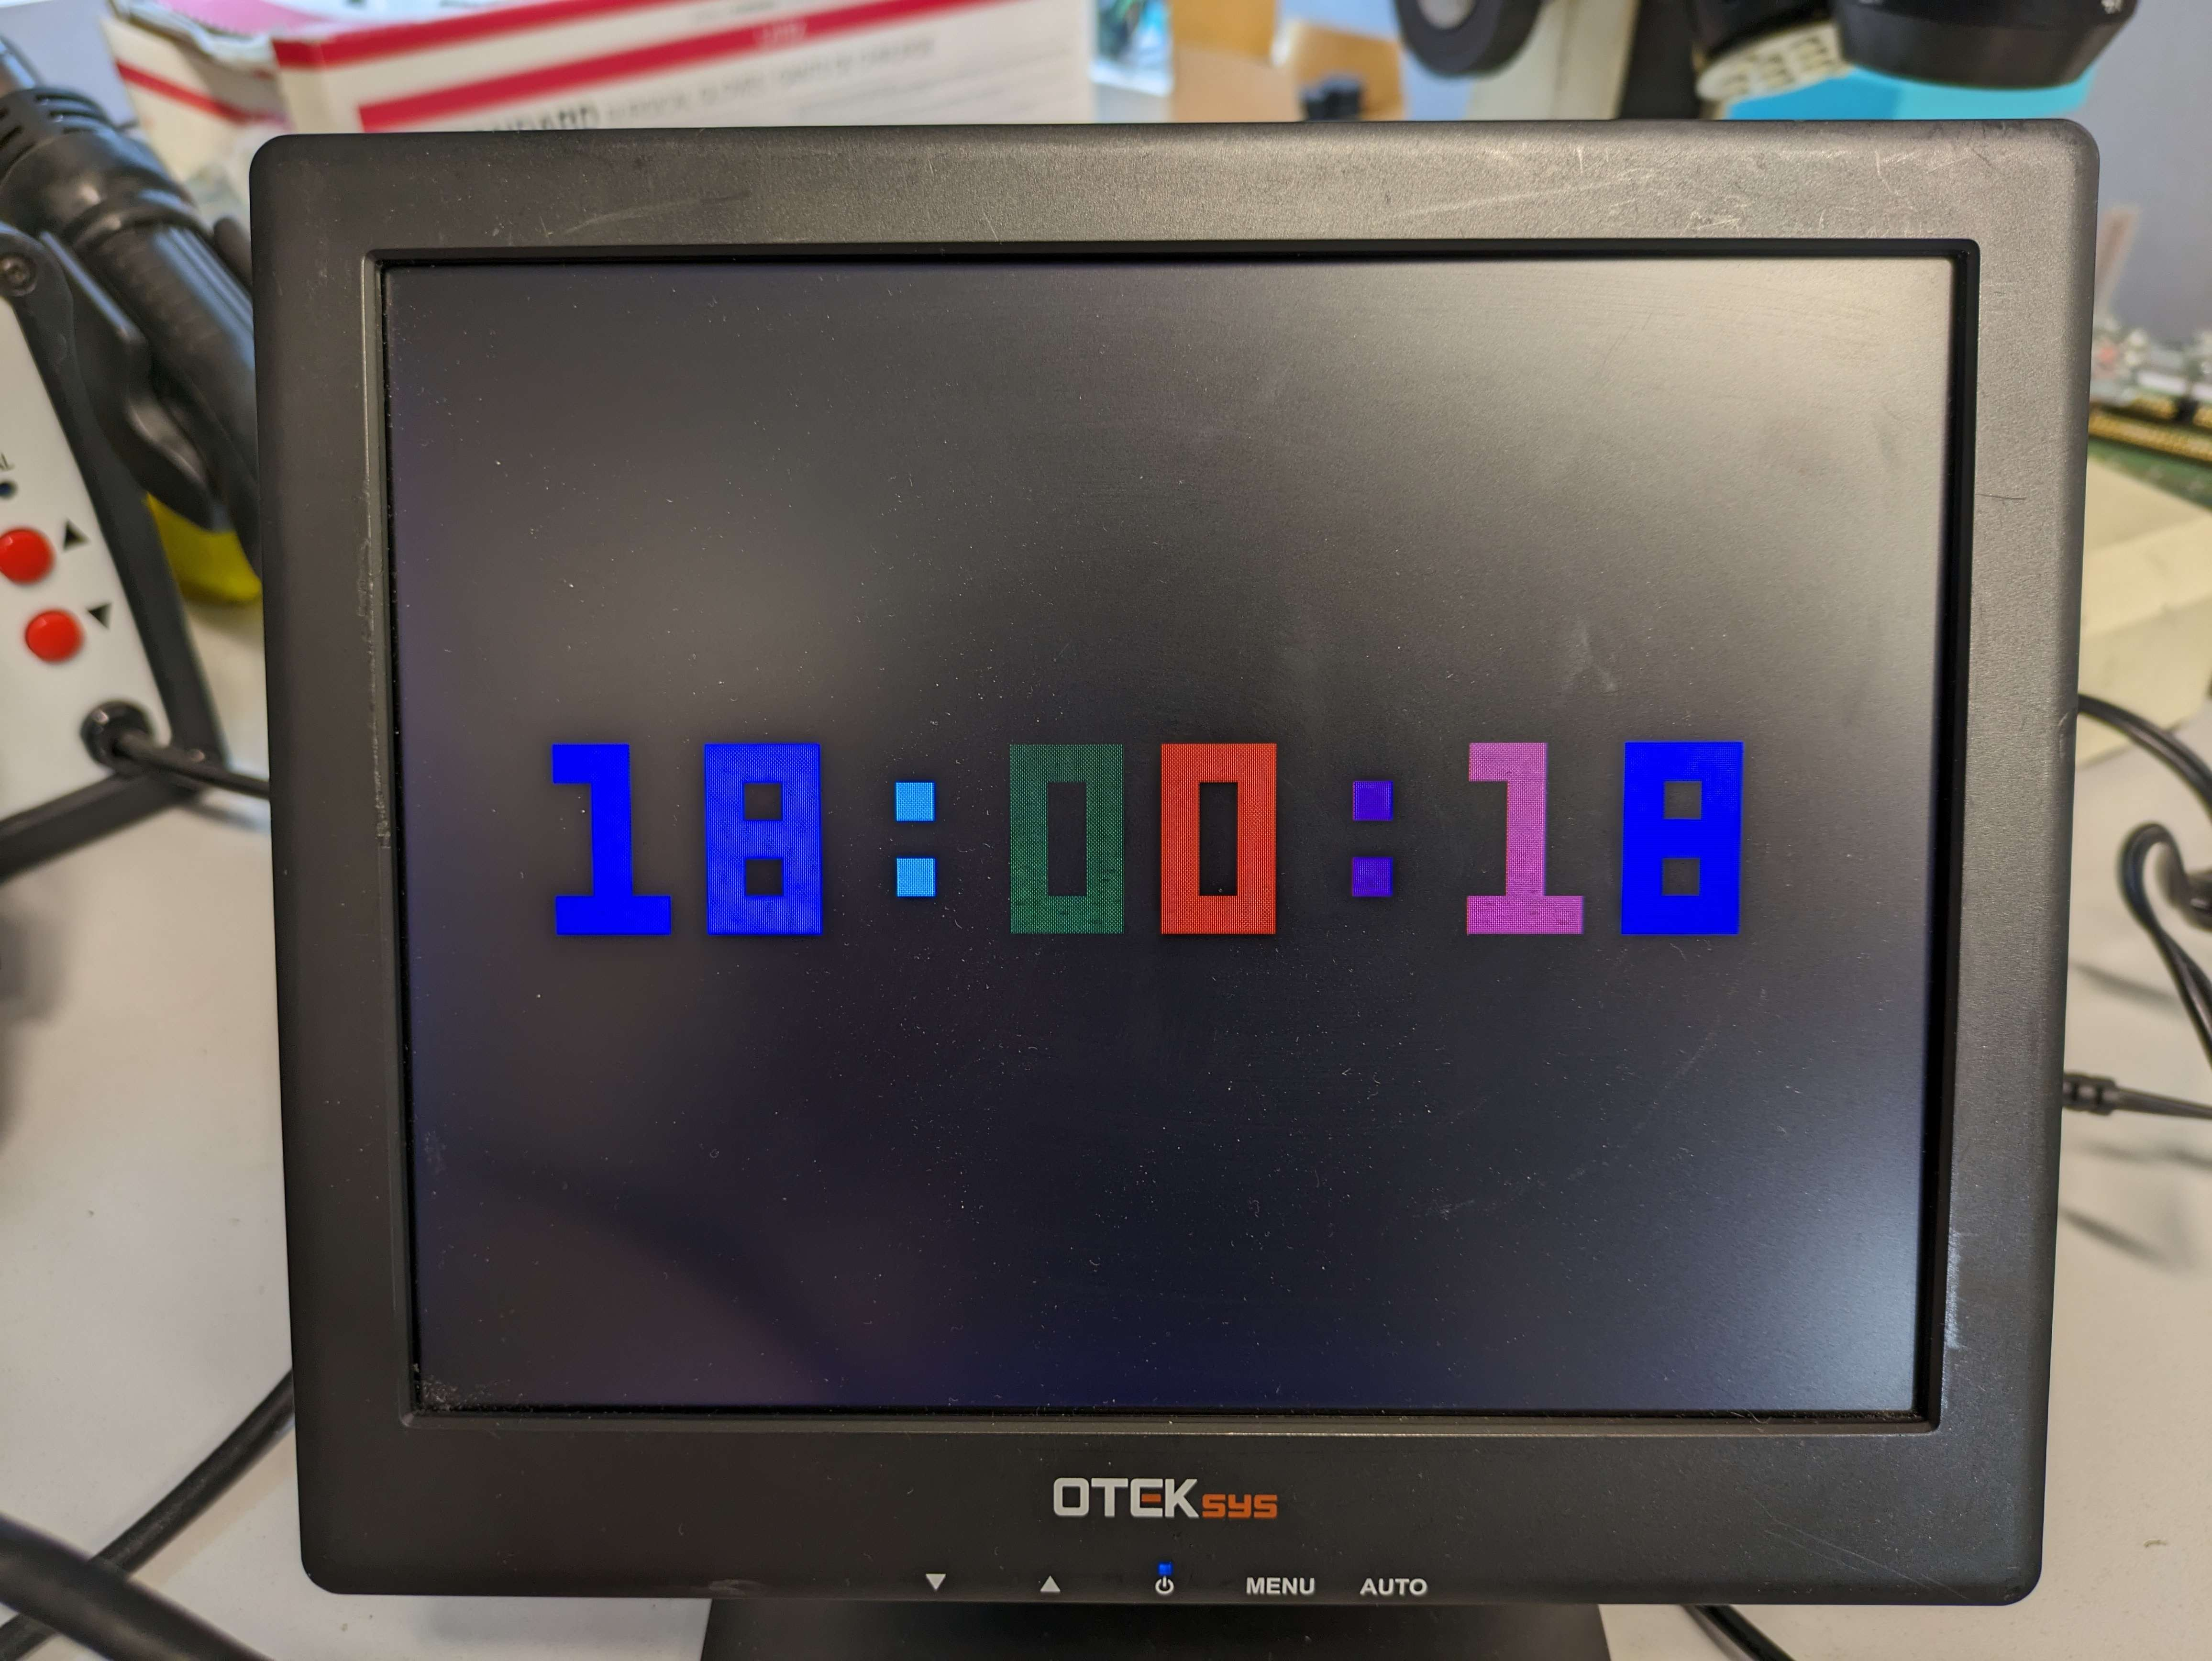
\includegraphics[width=\columnwidth]{./Figs/tt3p5 vga clock.jpg}
\caption{A VGA clock design running on Tiny Tapeout 3.5 silicon.}
\label{fig:VGA_clock_design_TT03_5_silicon}
\end{figure}

The new chip pinout and serial design selection required the creation of a new demonstration board (Fig.~\ref{fig:TT04plus_demo_board}), which was required to include an easy way to select a chosen design.
The Raspberry Pi RP2040 microcontroller was chosen as a coprocessor on the revised demonstration board, as it offers:

\begin{itemize}
\item Drag and drop firmware updates on any operating system,
\item MicroPython\cite{micropython} support, an ideal language and programming environment through which beginners can enable and test their designs (Fig.~\ref{fig:micropython_program}),
\item External memory emulation via programmable input output (PIO) and direct memory access (DMA) support.
\end{itemize}

\begin{figure}[!t]
\centering
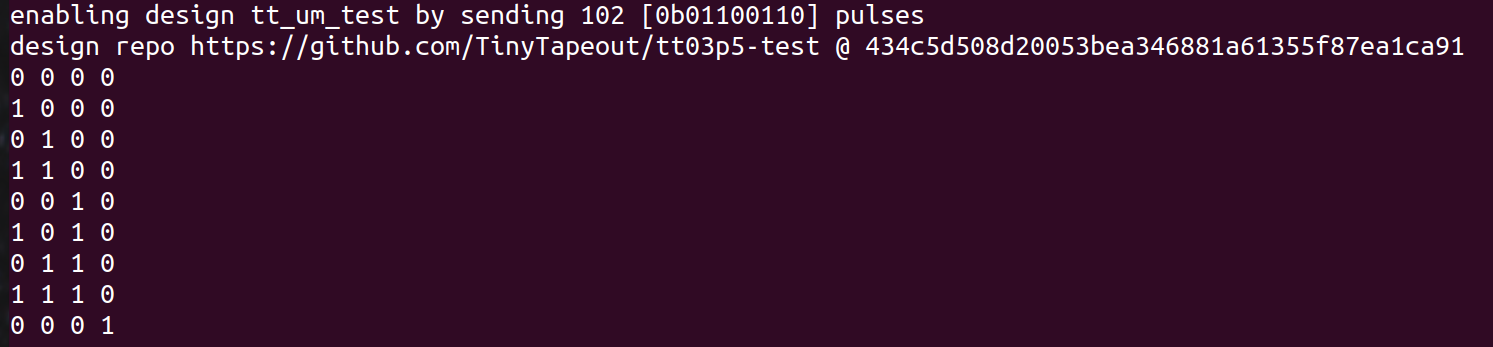
\includegraphics[width=\columnwidth]{./Figs/tt3p5 enable design.png}
\caption{A MicroPython program\cite{demofirmwaretest} enabling a chosen design, clocking it, and printing the results.}
\label{fig:micropython_program}
\end{figure}

\begin{figure}[!t]
\centering
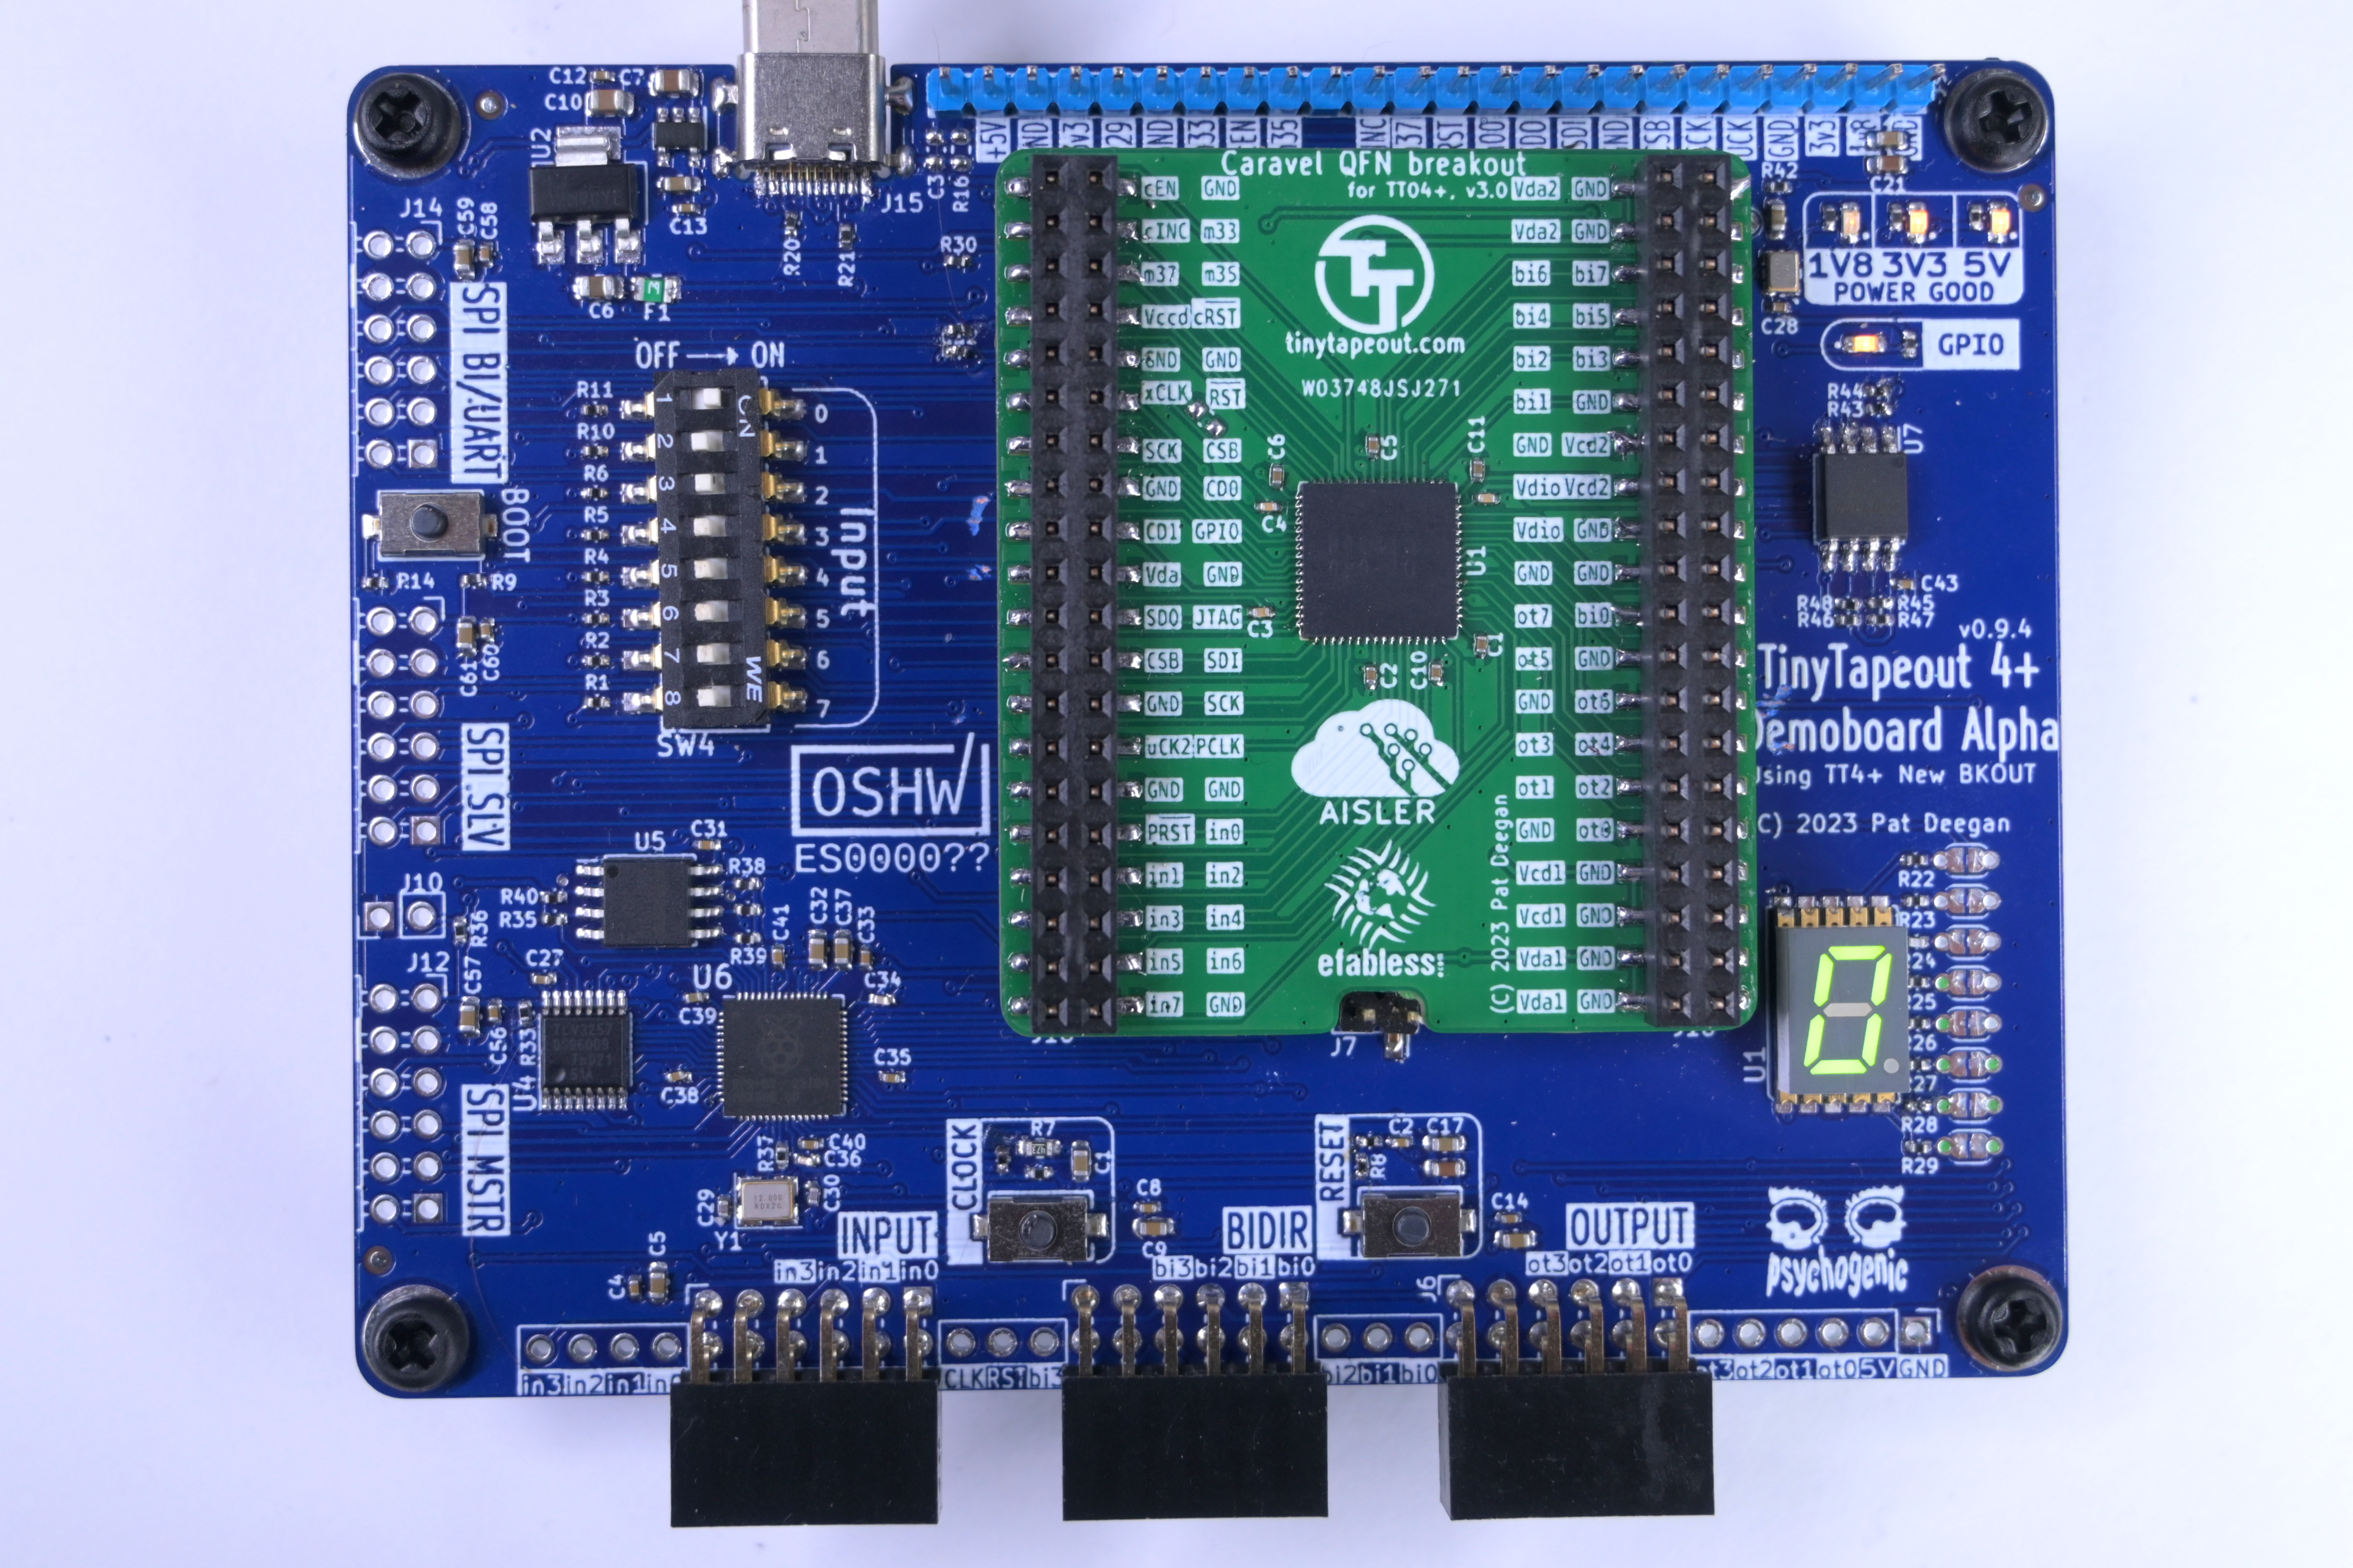
\includegraphics[width=\columnwidth]{./Figs/tt04-demoboard-top.jpg}
\caption{The Tiny Tapeout 4+ demonstration board\cite{tt04demoboard}.}
\label{fig:TT04plus_demo_board}
\end{figure}

An additional PMOD expansion port was added to the demonstration board for the bidirectional pins. The Tiny Tapeout community has begun to standardize on pinouts~\cite{pinouts}, making it easier to test each design.
A new repository was created to house user-contributed PMOD~\cite{awesomepmods} accessories, for example the VGA PMOD shown in Fig.~\ref{fig:user_contributed_VGA_PMOD}.

A further set of three PMOD expansion ports were added, mixing input and outputs, which allows the most common standard PMODs to be used with the demonstration board. For more information about the circuit board, pinout, and PMOD support see the repository~\cite{tt04demoboard}.

\begin{figure}[!t]
\centering
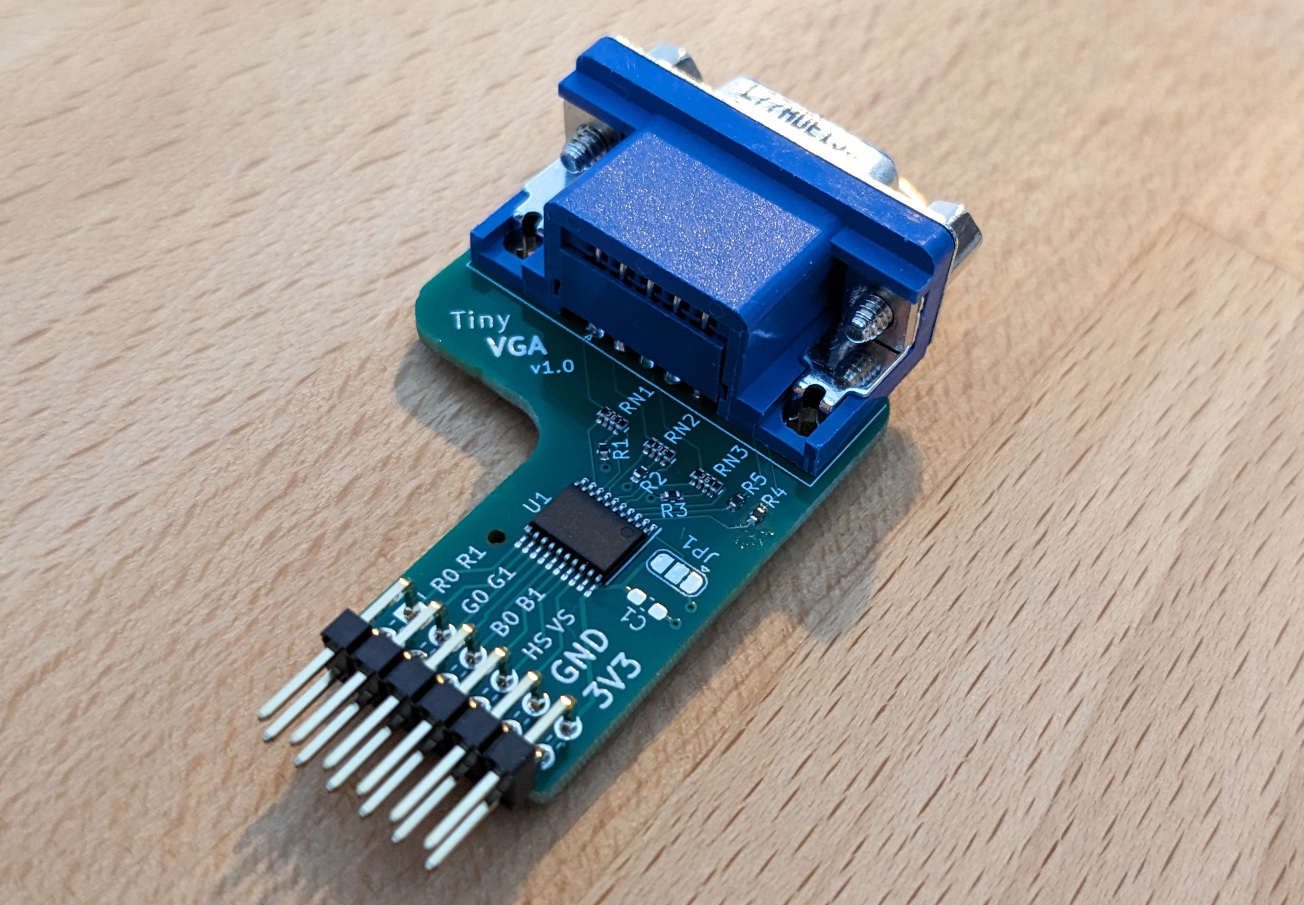
\includegraphics[width=\columnwidth]{./Figs/tiny_vga_pmod.jpg}
\caption{A user-contributed VGA output PMOD accessory for the demonstration board.}
\label{fig:user_contributed_VGA_PMOD}
\end{figure}
